\section{Process' Perspective}

\subsection{Developer interactions}
Throughout the development of the project during the course, the team has interacted primarily through Discord when remote communication was used. 
Further, the team met physically at ITU on Tuesdays where we communicated with each other during the entire day. 

\subsection{Team organization}
We organized ourselves as a cross-functional team. Sometimes we worked on tasks individually but for the majority of the project we worked together, 
typically in pairs. Every opinion and input from each team member was acknowledged equally. 

\subsection{CI/CD chains}
Our CI/CD chain consists of the following workflows used with GitHub Actions:
\begin{itemize}
    \item Continuous-deployment - Deploys the code of the main branch to production using Docker, ssh onto the server where we run our deployment script.
    \item Dev - Functions as the Continuous-deployment workflow but deploys to a test server.
    \item Test - Runs the test docker-compose file which creates a closed environment with the code on the current branch and runs the test.
    \item Main Release - This uses an extern workflow namely \textit{rymndhng/release-on-push-action@master} for creating a release every time a push to main is made.
    \item Lint - Uses the external workflow 'golangci/golangci-lint-action@v3' which checks the code with multiple linters.
\end{itemize}

Every time a pull request was made to a branch, the 'Lint' and 'Test' workflows were run. The workflows that handled deployment were triggered manually.
Further, we have set up CodeClimate and SonarCloud to help us maintain an appropriate standard of our code base such that we don't introduce new issues
with new features. The SonarCloud check is made every time a pull request is made to our main branch (see section \ref{branching} for a description of the 
branching structure).

\subsection{Organization of Repository}
The project only consists of a single repository containing the application. This repository contains several folders, 
each containing different files:

\renewcommand{\arraystretch}{3}
\begin{table}[H]
    \centering
    \resizebox{\textwidth}{!}{%
    \begin{tabular}{|l|l|}
    \hline
    \Large\textbf{.github/workflows} & \Large Contains all our workflow files used with GitHub Actions.                                                                                                          \\ \hline
    \Large\textbf{api\_test}         & \Large Includes files to run the simulator and a test of the API. Primarily used during the development of the endpoints.                                                     \\ \hline
    \Large\textbf{remote\_files}     & \Large Has all files that are used when deploying to the server. This includes various logging and monitoring files, \\ & \Large our deploy script, and the docker-compose file.      \\ \hline
    \Large\textbf{report}            & \Large This folder is where our report files are saved.                                                                                                                   \\ \hline
    \Large\textbf{src}               & \Large Contains all our application code which is further divided into subfolders, thereby separating the logic \\ & \Large of the system.                                            \\ \hline
    \Large\textbf{tests}             & \Large Our test files are located in this folder. It contains a Docker file, a docker-compose file, and a test file to \\ &  \Large run our tests without external impact. \\ \hline
    \end{tabular}%
    }
    \caption{Repository folders}
    \label{tab:repo_folders}
    \end{table}

\subsection{Branching strategy} \label{branching}
We used two static branches as part of our branching strategy throughout the development of the project. 
The main branch was used as our primary branch on which only functioning and tested code was meant to be pushed. It was
also the code on this branch we deployed on our main server. The other branch was the dev branch. This was used for 
development and testing. Additional branches were created when new functionality should be implemented, or bugs had to be
fixed. All these temporary branches were derived from the main branch. Our general branching strategy and an example where
we have used this in Github can be seen in figure \ref{fig:gen_branch} and \ref{fig:ex_branch}, respectively:

\begin{figure}[H]
    \centering
    \captionsetup{justification=centering,margin=1cm}
    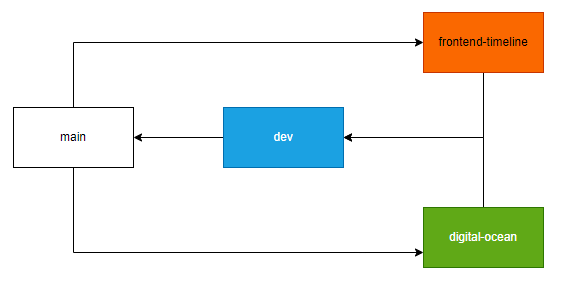
\includegraphics[width=0.7\linewidth]{report/images/branching.png}
    \caption{General branching strategy}
    \label{fig:gen_branch}
\end{figure}

\begin{figure}[H]
    \centering
    \captionsetup{justification=centering,margin=1cm}
    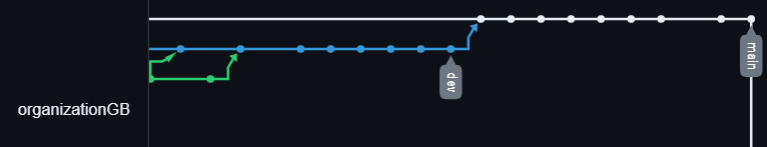
\includegraphics[width=0.7\linewidth]{report/images/git_branching.png}
    \caption{Example use of branching strategy}
    \label{fig:ex_branch}
\end{figure}

It can be seen that the temporary branches are derived from the main branch, and when the functionality is implemented, 
it is merged into the dev branch to be tested before the code is put into production. 

\subsection{Development process and tools}
Usually, when meeting on Tuesdays we discussed what needed to be done if we weren't already working on a task. We tried to start using a Kanban board but due to us not establishing 
clear guidelines on how to use the tool, we didn't manage to successfully implement it. In our development process, we utilized pair programming a lot. This also lead to a very iterative development 
process in the sense that we pushed small changes often to switch programmer. Further, the team agreed that when larger new implementations were to be introduced
to the main or dev branch, a pull request should be made to allow another team member to review the code and ensure that the workflows would catch any newly
introduced issues. 

\subsection{Monitoring}
The deployed MiniTwit application was monitored using Grafana, which is a dashboard web application for visualization of data. 
We used Grafana to monitor the simulator's interaction with our application and other parameters of the system. On our dashboard, 
we included a visualization of the CPU load percentage as well as an overview of the duration of requests to the different endpoints  
we got. Here it was possible to select a single endpoint and see the metrics for that type of request. This allowed us to analyze why 
there were higher CPU loads sometimes as this might be due to a resource-intensive request. Additionally, we monitored the total number of
responses to allow us to monitor the availability of the application. \\

To collect this data for visualization, we used Prometheus as it is an open-source monitoring system that can be used to collect 
and store various metrics data from the web server. Prometheus pulls the metric data from the MiniTwit application from an exposed metrics endpoint
and stores it so it can be queried by Grafana and shown in the dashboard.  

\subsection{Logging}
Not finished yet

\subsection{Security assessment}
From our security assessment, we learned that the risks with the highest likelihood were that an attacker could gain unauthorized access to our codebase
and our weak authentication and authorization mechanisms. The first risk was likely to occur as it was possible to find passwords and usernames for the database 
in our public codebase. We made sure that these are not stored directly in the source code by importing them from GitHub secrets instead. The second identified 
risk could be improved by changing the default usernames and passwords used to something that follows security standards.  

\subsection{Scaling and load balancing}
%Docker swarms and 2x nginx as load balancers. 
Not finished yet.

\subsection{AI-assistants}
The team has used AI-assistants to aid in the development and deployment of the MiniTwit application. We used OpenAI's ChatGPT, which is an AI language model, 
and Phind, which is an AI search engine. They were used to provide general information regarding the technologies we used as well as how to approach development tasks,
such as describing the different components used in a docker-compose file or implementing a Go application using the Gin framework. \\
  
Using these assistants aided us because they provided a quick overview of the possibilities with short explanations. They gave us a way to quickly get started with
implementation in a language we did not know as it suggested code in which we were quickly able to learn the syntax of Go and how to structure our application. However, 
using them also hindered us as we often had to double-check whether the information provided was accurate and so ended up using more time than if we obtained the information 
without them. 